\subsection{Chức năng nhắn tin riêng tư (Private message)}
\subsubsection{Use case}

\begin{table}[H]
    \centering
    \begin{tabular}{|l|p{11cm}|}
        \hline
        Category & Description \\
        \hline
        Use case name & Private message \\
        \hline
        Actor & Sinh viên \\
        \hline
        Assumption & Người dùng đang ở đường dẫn \url{https://school.moodledemo.net/}. Ngôn ngữ của trang web được chỉnh là Tiếng Việt. \\ 
        & - User 1 username: amandahamilto205, password: moodle\\
        & - User 2 username: student, password: moodle\\
        &Người dùng đăng nhập thành công dưới tài khoản sinh viên. Người dùng đang ở trang "Trang chủ".\\\hline
        Normal flow & 
        1. Ở trang chủ, user 1 click biểu tượng Chat. \\
        & 2. Hệ thống hiển thị khung chat nhỏ trên màn hình. \\
        & 3. User 1 chọn user 2 trong mục Riêng tư trên khung chat nhỏ.\\
        & 4. Hệ thống hiển thị lịch sử chat.\\
        & 5. User 1 gõ tin nhắn văn bản, icon vào ô chat và nhấn gửi.\\
        & 6. Hệ thống hiển thị tin nhắn user 1 vừa gửi trên chatbox.\\
        & 7. Hệ thống gửi tin nhắn và hiển thị thông báo đến user 2.\\\hline
        Alternative flows &
        A1. Tại bước 5:\\
        & 5.1 Người dùng nhấn chọn tin nhắn.\\
        & 5.2 Người dùng chọn icon Xóa những tin nhắn được chọn.\\
        & 5.3 Người dùng xác nhận Xóa.
        \\\hline
        Exception flows &
        E1. Tại bước 5:\\
        & 5.1 Người dùng gửi tin nhắn với độ dài 4100 kí tự.\\
        & 5.2 Hệ thống giới hạn độ dài tin nhắn 4096 kí tự và không có phép gõ nữa.\\ & \\
        & E2. Tại bước 6, nếu user 2 đã block user 1\\
        & 6.1: Hệ thống hiển thị lỗi không gửi được tin nhắn cho user 2.\\\hline
    \end{tabular}
    \caption{Use case: Private message}
    \label{tab:Private-message}
\end{table}

\subsubsection{Activity diagram}
\begin{figure}[H]
    \centering
    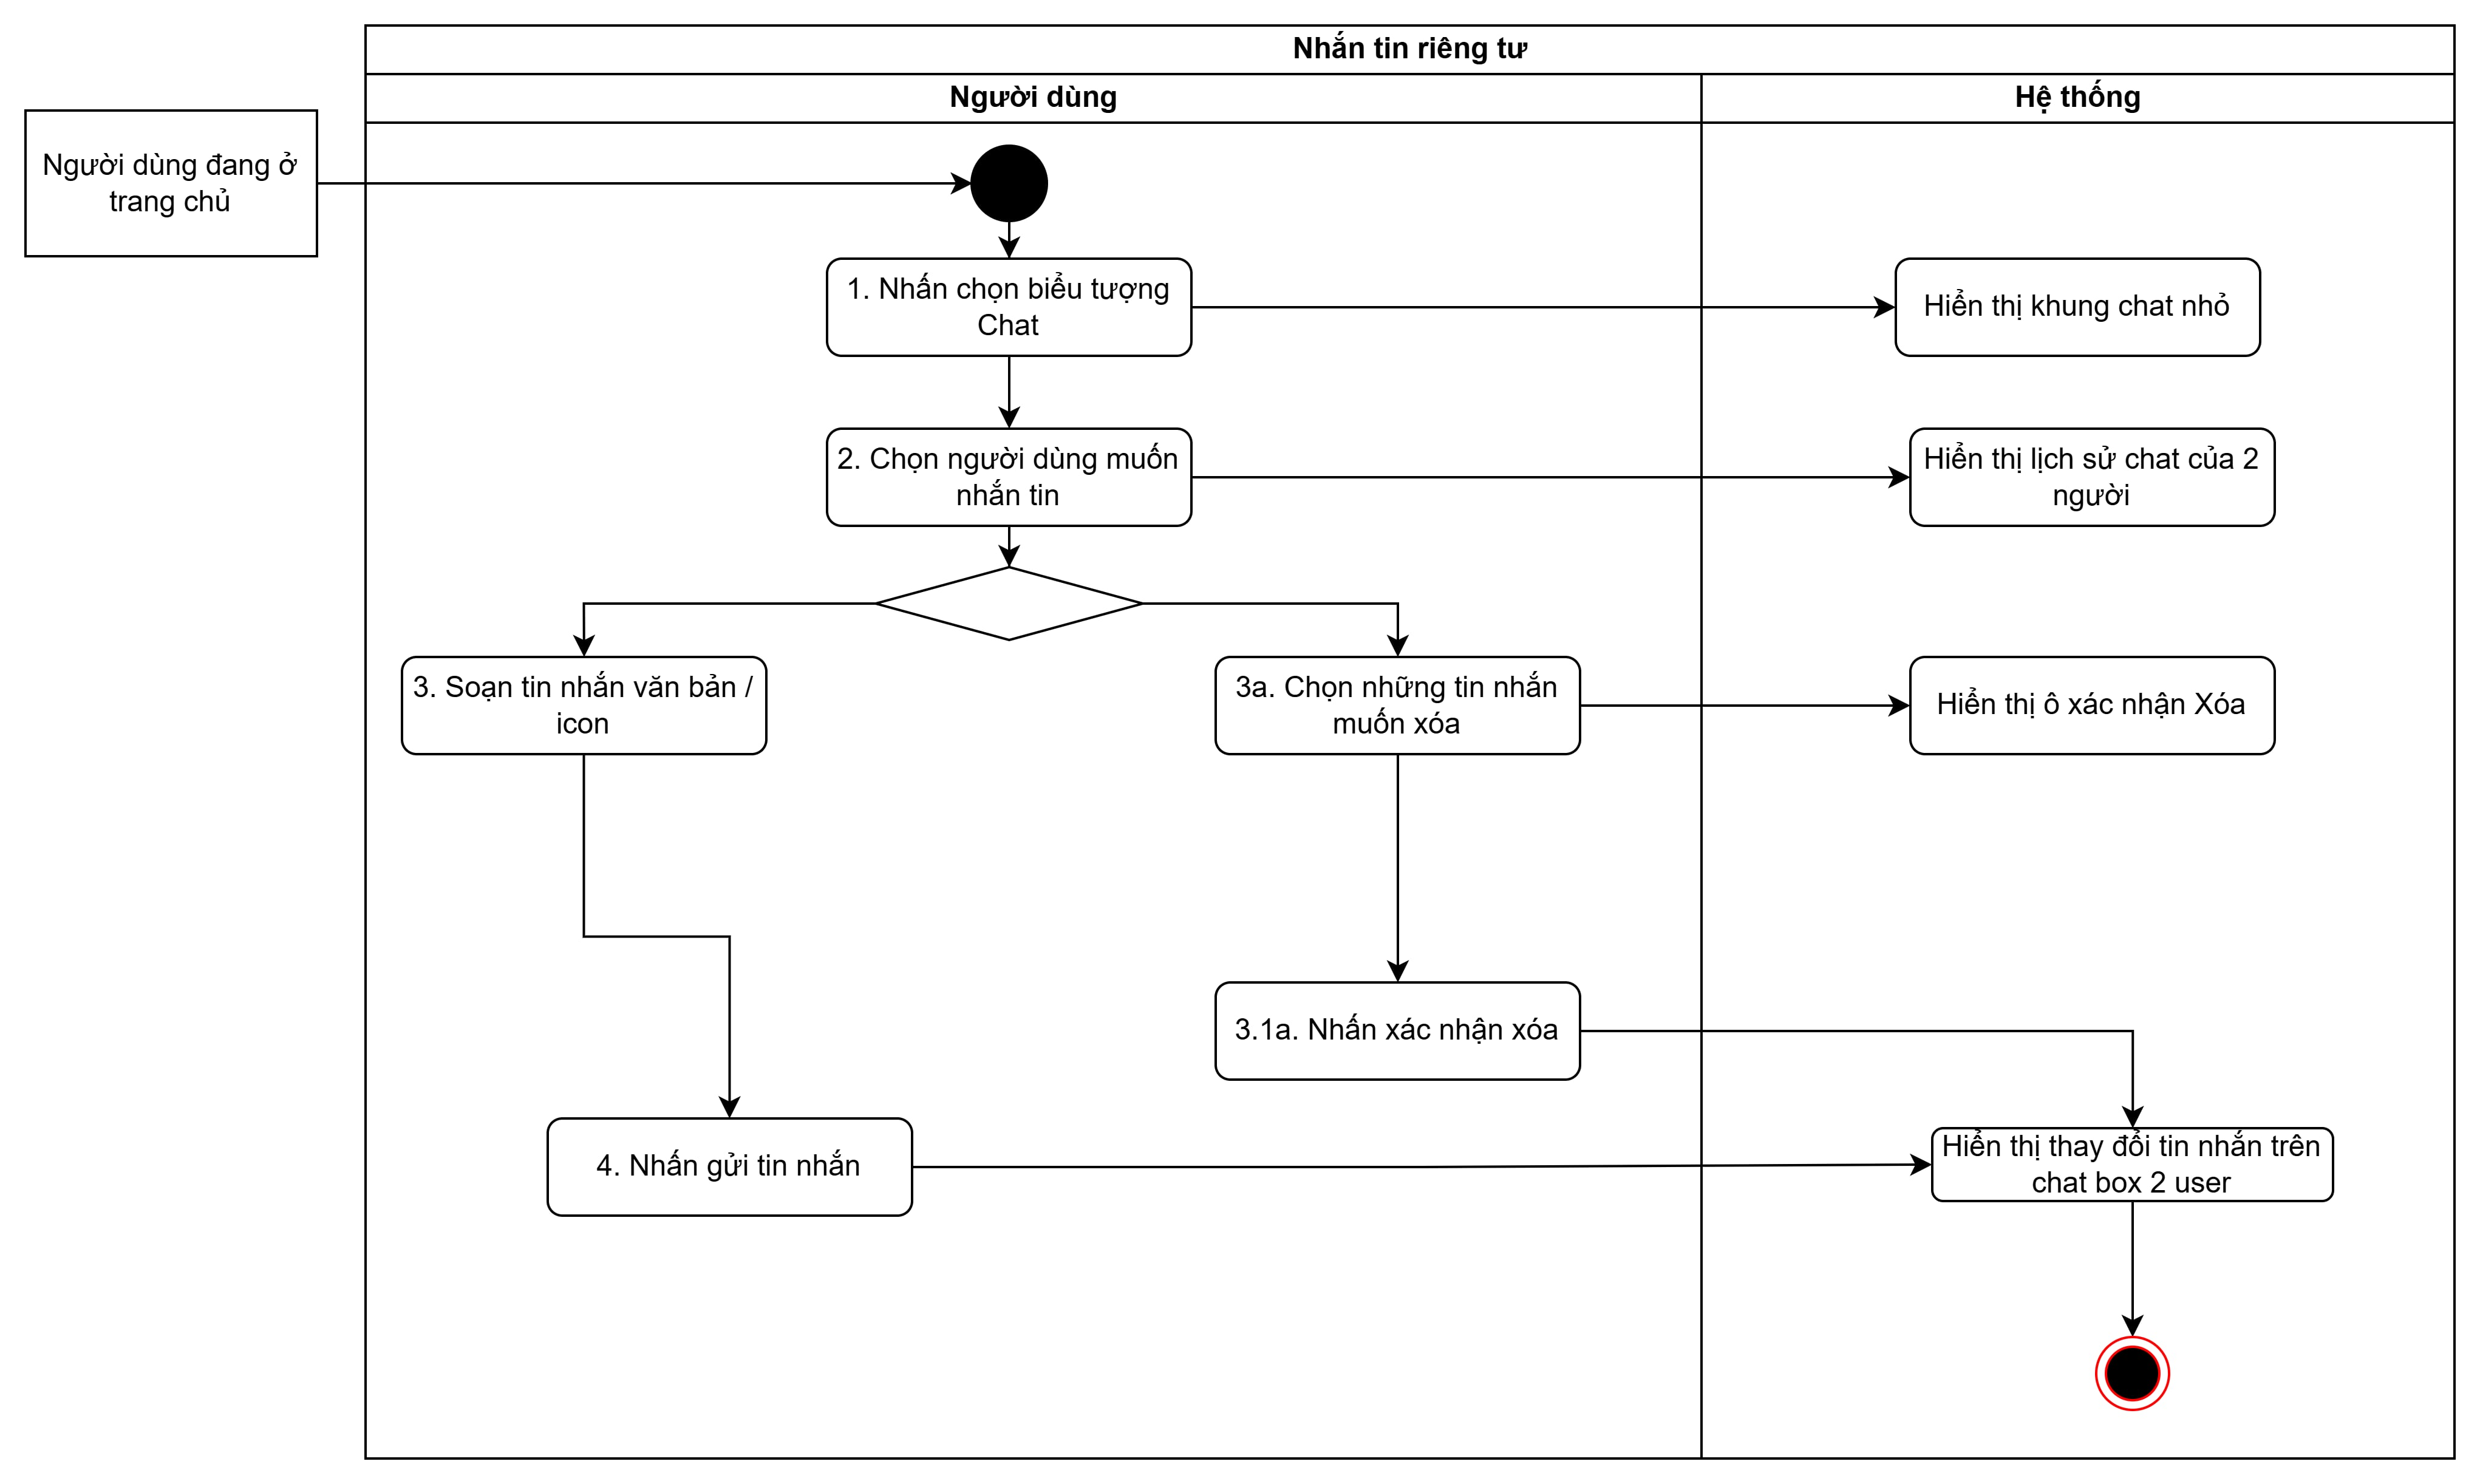
\includegraphics[width=\textwidth]{image/private-message.png}
    \caption{Activity diagram for Private message}
    \label{fig:activity-diagram-private-message}
\end{figure}
\subsubsection{Sử dụng phương pháp Boundary value analysis để kiểm thử}
Ta chọn Normal Boundary Value testing, dựa theo các lí do sau:
\begin{itemize}
    \item Giới hạn số lượng kí tự tin nhắn là 1 phạm vi liên tục với biên rõ ràng, lựa chọn BVA phù hợp để kiểm thử các giá trị tại biên, gần biên.
    \item Kiểm tra giá trị biên giúp đảm bảo rằng hệ thống xử lý đúng các tình huống cận biên, nơi dễ phát sinh lỗi nhất.
\end{itemize}
Thay giá trị input ở bước 5 theo domain như sau, gọi x là "Số lượng kí tự input" \(1\ \text{kí tự} \leq x \leq 4096\ \text{kí tự}\).
\begin{itemize}
    \item PM-001-001: Gửi tin nhắn với số lượng kí tự từ 1 - 4096.
    \item PM-001-002: Gửi tin nhắn với số lượng kí tự tối thiểu.
    \item PM-001-003: Gửi tin nhắn với số lượng kí tự tối thiểu +.
    \item PM-001-004: Gửi tin nhắn với số lượng kí tự tối đa.
    \item PM-001-005: Gửi tin nhắn với số lượng kí tự tối đa -.
\end{itemize}
\subsubsection{Sử dụng phương pháp Equivalence class partitioning}
Lí do chọn: Chức năng gửi tin nhắn riêng tư có số lượng kí tự giới hạn dựa trên một phạm vi kích thước liên tục rõ ràng (1 kí tự - 4096 kí tự). Có thể dễ dàng chia ra lớp tương đương hợp lệ và không hợp lệ.. \\
Thực hiện Weak Normal Equivalence Class Testing, chia input ở bước 5 thành các equivalence class như sau:
\begin{itemize}
    \item "Số lượng kí tự" gọi là x, ta chia thành 1 class valid: \(1\ \text{kí tự} \leq x \leq 4096\ \text{kí tự}\), 2 class invalid là \(x < 1\ \text{kí tự}\) và \(x > 4096\ \text{kí tự}\).
\end{itemize}
Test case:
\begin{itemize}
    \item PM-002-001: Gửi tin nhắn với số lượng < 1 kí tự.
    \item PM-002-002: Gửi tin nhắn với số lượng > 4096 kí tự.
    \item PM-001-001: Gửi tin nhắn với số lượng kí tự từ 1 - 4096.
\end{itemize}

\subsubsection{Sử dụng phương pháp Decision table để kiểm thử}

\begin{table}[H]
    \centering
    \begin{tabular}{|l|c|c|c|c|}
        \hline
        \textbf{Điều kiện} & \textbf{1} & \textbf{2} & \textbf{3} & \textbf{4} \\
        \hline
        c1. Tin nhắn có số lượng kí tự hợp lệ & Có & Không & Có & Không \\
        \hline
        c2. Người nhận không chặn người gửi & Có & Có & Không & Không \\\hline
        \textbf{a1. Thành công gửi} & x & & & \\
        \hline
        \textbf{a2. Tin nhắn không được gửi} & & x & x &x \\
        \hline
    \end{tabular}
    \caption{Bảng quyết định kiểm thử chức năng nhắn tin riêng tư}
    \label{tab:decision-table-private-message}
\end{table}
Tương ứng với bảng quyết định trên, ta có các test case:
\begin{itemize}
    \item PM-004-001: Gửi tin nhắn hợp lệ, người nhận không chặn.
    \item PM-004-002: Gửi tin nhắn không hợp lệ, người nhận không chặn.
    \item PM-004-003: Gửi tin nhắn không hợp lệ, người nhận chặn.
    \item PM-004-004: Gửi tin nhắn hợp lệ, người nhận chặn.
\end{itemize}
\subsubsection{Sử dụng phương pháp Use-case testing để kiểm thử}
Dựa theo Activity diagram, ta chia thành các path:
\begin{itemize}
    \item P1: 1,2,3,4 tương ứng với PM-001-001
    \item P2: 1,2,3a,3.1a tương ứng với PM-003-001
\end{itemize}
\newpage